\documentclass[letterpaper,12pt]{article}
\usepackage{array}
\usepackage{threeparttable}
\usepackage{geometry}
\geometry{letterpaper,tmargin=1in,bmargin=1in,lmargin=1.25in,rmargin=1.25in}
\usepackage{fancyhdr,lastpage}
\pagestyle{fancy}
\lhead{}
\chead{}
\rhead{}
\lfoot{}
\cfoot{}
\rfoot{\footnotesize\textsl{Page \thepage\ of \pageref{LastPage}}}
\renewcommand\headrulewidth{0pt}
\renewcommand\footrulewidth{0pt}
\usepackage[format=hang,font=normalsize,labelfont=bf]{caption}
\usepackage{listings}
\lstset{frame=single,
  language=Python,
  showstringspaces=false,
  columns=flexible,
  basicstyle={\small\ttfamily},
  numbers=none,
  breaklines=true,
  breakatwhitespace=true
  tabsize=3
}
\usepackage{amsmath}
\usepackage{amssymb}
\usepackage{amsthm}
\usepackage{harvard}
\usepackage{setspace}
\usepackage{float,color}
\usepackage[pdftex]{graphicx}
\usepackage{hyperref}
\hypersetup{colorlinks,linkcolor=red,urlcolor=blue}
\theoremstyle{definition}
\newtheorem{theorem}{Theorem}
\newtheorem{acknowledgement}[theorem]{Acknowledgement}
\newtheorem{algorithm}[theorem]{Algorithm}
\newtheorem{axiom}[theorem]{Axiom}
\newtheorem{case}[theorem]{Case}
\newtheorem{claim}[theorem]{Claim}
\newtheorem{conclusion}[theorem]{Conclusion}
\newtheorem{condition}[theorem]{Condition}
\newtheorem{conjecture}[theorem]{Conjecture}
\newtheorem{corollary}[theorem]{Corollary}
\newtheorem{criterion}[theorem]{Criterion}
\newtheorem{definition}[theorem]{Definition}
\newtheorem{derivation}{Derivation} % Number derivations on their own
\newtheorem{example}[theorem]{Example}
\newtheorem{exercise}[theorem]{Exercise}
\newtheorem{lemma}[theorem]{Lemma}
\newtheorem{notation}[theorem]{Notation}
\newtheorem{problem}[theorem]{Problem}
\newtheorem{proposition}{Proposition} % Number propositions on their own
\newtheorem{remark}[theorem]{Remark}
\newtheorem{solution}[theorem]{Solution}
\newtheorem{summary}[theorem]{Summary}
%\numberwithin{equation}{section}
\bibliographystyle{aer}
\newcommand\ve{\varepsilon}
\newcommand\boldline{\arrayrulewidth{1pt}\hline}


\begin{document}

\begin{flushleft}
  \textbf{\large{Problem Set \#4}} \\
  MACS 40200, Dr. Evans \\
  Bobae Kang
\end{flushleft}

\vspace{5mm}

\begin{enumerate}
\item \textbf{Matching the U.S. income distribution by GMM.}
\begin{enumerate}
\item Plot the histogram implied by the moments in the tab-delimited text file \texttt{usincmoms.txt}.
\par
\begin{figure}[H]\centering\captionsetup{width=4.0in}
   \fbox{\resizebox{4.0in}{3.0in}{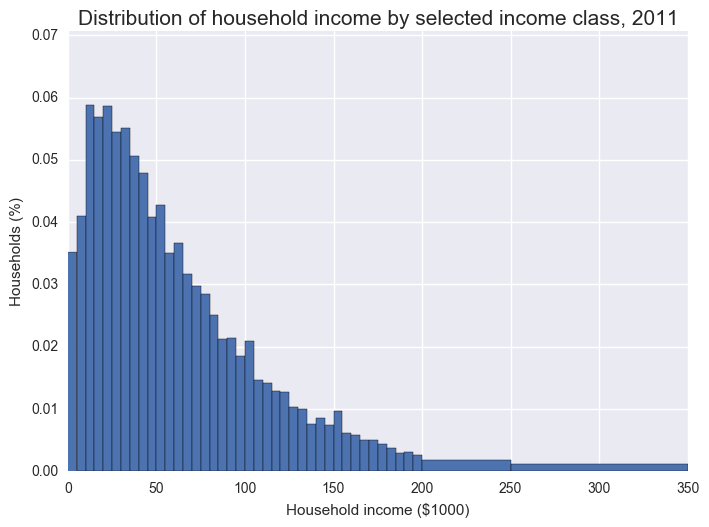
\includegraphics{./images/fig_1a.png}}}
\end{figure}
\par\bigskip

\item Using GMM, fit the lognormal LN(x; $\mu$, $\sigma$) distribution defined in the MLE notebook to the distribution of household income data using the moments from the data file. Report your estimated values for $\hat{\mu}$ and $\hat{\sigma}$, as well as the value of the minimized criterion function. Plot the histogram from part (a) overlayed with a line representing the implied histogram from your estimated lognormal (LN) distribution.
\par
\begin{figure}[H]\centering\captionsetup{width=4.0in}
  \fbox{\resizebox{4.0in}{3.0in}{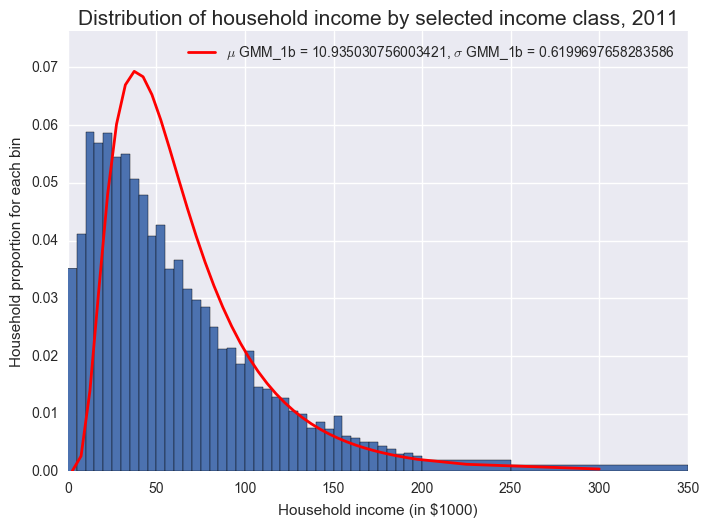
\includegraphics{./images/fig_1b.png}}}
\end{figure}
\par
GMM crietron function value: 0.04594528 \par
GMM estimate for $\mu$, with $\textbf{W}$: 10.76684402\par
GMM estimate for $\sigma$, with $\textbf{W}$: 0.90784121 \par
\bigskip

\item Using GMM, fit the gamma GA(x; $\alpha$, $\beta$) distribution defined in the MLE notebook to the distribution of household income data using the moments from the data file. Report your estimated values for $\hat{\alpha}$  and  $\hat{\beta}$, as well as the value of the minimized criterion function. Plot the histogram from part (a) overlayed with a line representing the implied histogram from your estimated gamma (GA) distribution.
\par
\begin{figure}[H]\centering\captionsetup{width=4.0in}
  \fbox{\resizebox{4.0in}{3.0in}{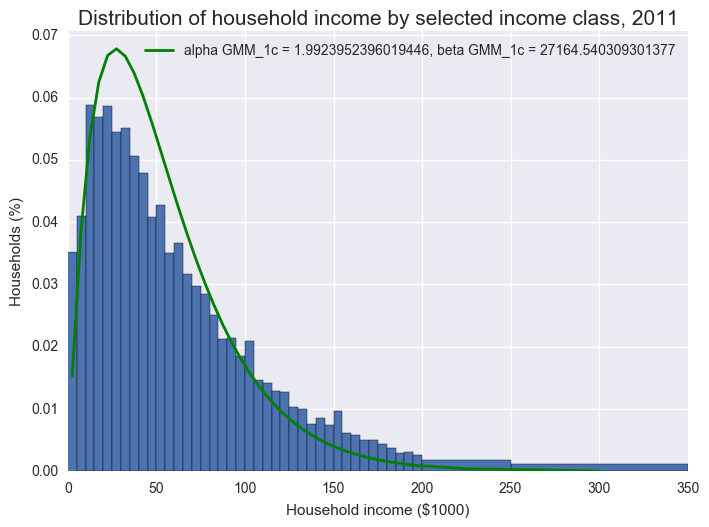
\includegraphics{./images/fig_1c.png}}}
\end{figure}
\par
GMM crietron function value: 0.0123431\par
GMM estimate for $\alpha$, with given $\textbf{W}$: 1.36141460361  \par
GMM estimate for $\beta$, with given $\textbf{W}$: 48380.3223213 \par
\bigskip

\item Plot the histogram from part (a) overlayed with the line representing the implied histogram from your estimated lognormal (LN) distribution from part (b) and the line representing the implied histogram from your estimated gamma (GA) distribution from part (c). What is the most precise way to tell which distribution fits the data the best? Which estimated distribution--LN or GA--fits the data best?
\par
\begin{figure}[H]\centering\captionsetup{width=4.0in}
  \fbox{\resizebox{4.0in}{3.0in}{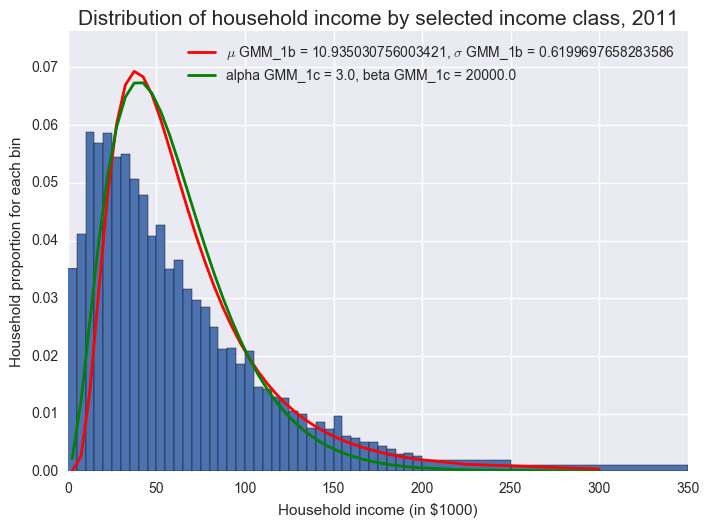
\includegraphics{./images/fig_1d.png}}}
\end{figure}
\par
As illustrated by the plot above, the GA distribution fits the data with greater precision than the LN distribution. In addition, using the weight matrix $\textbf{W} = \textbf{I}$, we can compare the criterion function values. This comparison also suggests that the GA distribution fits the data better.
\bigskip

\item Repeat your estimation of the GA distribution from part (c), but use the two-step estimator for the optimal weighting matrix. Do your estimates for $\alpha$ and $\beta$ change much? How can you compare the goodness of fit of this estimated distribution versus the goodness of fit of the estimated distribution in part (c)?
\par
\begin{figure}[H]\centering\captionsetup{width=4.0in}
  \fbox{\resizebox{4.0in}{3.0in}{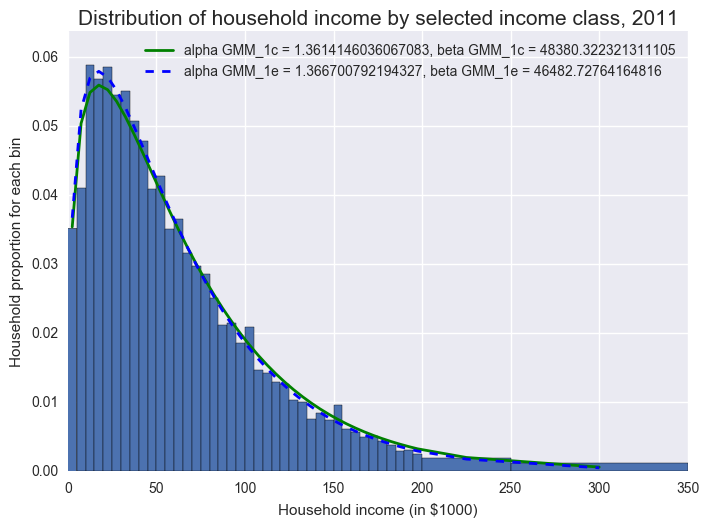
\includegraphics{./images/fig_1e.png}}}
\end{figure}
\par
GMM crietron function value: 1.21083883e+08\par
GMM estimate for $\alpha$, with $\hat{\textbf{W}}_{twostep}$: 1.36670079219 \par
GMM estimate for $\beta$, with $\hat{\textbf{W}}_{twostep}$: 46482.7276416\par
\bigskip
The GMM estimates for $\alpha$ and $\beta$ did not change significantly. With the same initial input for parameters, the esitmate for $\alpha$ changed from 1.361 to 1.367, and the estimate for $\beta$ from 48380.322 to 46482.728. The different weight matrices make it not ideal for me to simply compare the criterion function values. The plot suggests that the first GMM estimates with the given weighting matrix $\textbf{W}$ fits the distribution to the data almost as well as the second estimates with the two-step weighting matrix, $\hat{\textbf{W}}_{twostep}$. 
\end {enumerate}
\end {enumerate}

\end{document}
